\documentclass[12pt,a4paper]{article}

%% ------------------------------------------------------------------
%% Packages
%% ------------------------------------------------------------------
\usepackage[utf8]{inputenc}
\usepackage[T1]{fontenc}
\usepackage[english]{babel}
\usepackage{geometry}
\usepackage{amsmath}
\usepackage{amssymb}
\usepackage{booktabs}
\usepackage{array}
\usepackage{longtable}
\usepackage{graphicx}
\usepackage{float}
\usepackage{caption}
\usepackage{subcaption}
\usepackage{hyperref}
\usepackage{xcolor}
\usepackage{listings}
\usepackage{parskip}
\usepackage{enumitem}
\usepackage{titlesec}
\usepackage{fancyhdr}
\usepackage{multirow}
\usepackage{makecell}

\geometry{
  top=2.5cm,
  bottom=2.5cm,
  left=3cm,
  right=3cm,
}

%% ------------------------------------------------------------------
%% Colors and hyperref
%% ------------------------------------------------------------------
\definecolor{linkblue}{RGB}{37,99,235}
\definecolor{codeblue}{RGB}{99,102,241}
\definecolor{codebg}{RGB}{248,250,252}
\definecolor{best}{RGB}{22,163,74}       % green for best values
\definecolor{secbest}{RGB}{234,88,12}    % orange for 2nd best

\hypersetup{
  colorlinks=true,
  linkcolor=linkblue,
  urlcolor=linkblue,
  citecolor=linkblue,
  pdftitle={Week 12: Graph Analytics and Centrality Report},
  pdfauthor={Grupo 06 --- Big Data},
}

%% ------------------------------------------------------------------
%% Code listings
%% ------------------------------------------------------------------
\lstset{
  basicstyle=\ttfamily\footnotesize,
  backgroundcolor=\color{codebg},
  frame=single,
  rulecolor=\color{gray!30},
  breaklines=true,
  columns=flexible,
  keywordstyle=\color{codeblue}\bfseries,
  commentstyle=\color{gray},
  stringstyle=\color{teal},
}

%% ------------------------------------------------------------------
%% Header / footer
%% ------------------------------------------------------------------
\pagestyle{fancy}
\fancyhf{}
\rhead{Grupo 06 --- Big Data}
\lhead{Week 12: Graph Analytics}
\rfoot{\thepage}

%% ------------------------------------------------------------------
%% Title
%% ------------------------------------------------------------------
\title{
  \vspace{-1cm}
  \Large\textbf{Week 12 Milestone Report}\\[0.4em]
  \large Graph Analytics and Centrality Report\\[0.3em]
  \normalsize MovieLens Discovery System --- Semester Project
}
\author{
  Grupo 06 --- Big Data\\
  \texttt{BD-Grupo-06/movielens-discovery}
}
\date{\today}

%% ==================================================================
\begin{document}
%% ==================================================================

\maketitle
\thispagestyle{fancy}
\tableofcontents
\newpage

%% ------------------------------------------------------------------
\section{Executive Summary}
%% ------------------------------------------------------------------

This report covers Week~12: formalizing the item-item graph induced by the MovieLens catalog and
using it for structural analysis. The graph reuses the Week~10 SVD item-factor space (the same
signal behind the \texttt{svd\_collaborative} recommender), so this is a genuine structural view of
an existing signal, not an unrelated ad hoc graph.

\begin{table}[H]
\centering
\caption{Graph overview and headline validity/comparison numbers}
\begin{tabular}{ll}
\toprule
\textbf{Metric} & \textbf{Value} \\
\midrule
Nodes & 13,176 (movies with $\geq50$ ratings, i.e.\ a Week~10 SVD item factor) \\
Edges & 155,331 (undirected, weighted by cosine similarity) \\
Sparsity & 0.179\% of all possible pairs \\
Isolated nodes & 29 (0.22\%) \\
Connected components & 33 \\
Giant component coverage & 13,139 nodes (\textbf{99.72\%}) \\
Spearman $\rho$: popularity vs.\ graph PageRank & \textbf{0.313} \\
Spearman $\rho$: model rec.\ in-degree vs.\ graph PageRank & \textbf{0.578} \\
\bottomrule
\end{tabular}
\end{table}

The graph is highly connected (one dominant component covering 99.7\% of nodes) at the chosen
configuration ($k=15$ neighbors, minimum cosine similarity $0.5$). PageRank correlates only weakly
with raw popularity ($\rho=0.313$), confirming that graph centrality captures something
structurally different from ``most-rated'' --- a small number of niche, low-popularity titles are
highly central because their rating pattern places them in a densely interconnected similarity
neighborhood.

%% ------------------------------------------------------------------
\section{Objective}
%% ------------------------------------------------------------------

The goal of Week~12 was to formalize the domain as a graph and use it for structural analysis,
connecting back to the Week~10 recommendation layer rather than building an unrelated graph:

\begin{quote}
  \textit{What does the similarity structure among movies look like as a graph, and does structural
  centrality tell us something different from popularity or model-based ranking?}
\end{quote}

Specific questions addressed:
\begin{itemize}[nosep]
  \item What do nodes and edges mean, and why are they defined this way?
  \item Is the chosen graph configuration ($k$, similarity threshold) robust, or a hand-picked lucky run?
  \item Does PageRank on the similarity graph rank movies differently than popularity or the
    Week~10 recommender's in-degree?
  \item What does high centrality mean in this domain, and --- just as important --- what does it
    \emph{not} mean?
\end{itemize}

%% ------------------------------------------------------------------
\section{Inputs and Reproducible Artifacts}
%% ------------------------------------------------------------------

\subsection{Input artifacts from previous weeks}

\begin{table}[H]
\centering
\caption{Inputs consumed from prior weeks}
\begin{tabular}{lll}
\toprule
\textbf{Artifact} & \textbf{Source} & \textbf{Purpose} \\
\midrule
\texttt{week10\_svd\_item\_factors.parquet} & Week~10 & 50-dim item factors: node features / edge weights \\
\texttt{week10\_popularity\_global.csv} & Week~10 & Popularity ranking (comparison baseline) \\
\texttt{week10\_svd\_recs\_top20.parquet} & Week~10 & Recommendation in-degree (model-based baseline) \\
\texttt{week07\_kmeans\_assignments.csv} & Week~7 & Cluster labels for the web viewer \\
\texttt{movies\_catalog.parquet}, \texttt{links.csv} & Week~3 & Titles, genres, IMDb/TMDb IDs \\
\bottomrule
\end{tabular}
\end{table}

\subsection{Week 12 output artifacts}

\begin{table}[H]
\centering
\caption{Output artifacts produced in Week~12}
\begin{tabular}{ll}
\toprule
\textbf{File} & \textbf{Description} \\
\midrule
\texttt{week12\_graph\_meta.json} & Graph definition, chosen configuration, validity checks, correlations \\
\texttt{week12\_graph\_metrics.parquet} & Per-node degree, weighted degree, PageRank, eigenvector, betweenness \\
\texttt{week12\_sensitivity\_sweep.csv/.html/.png} & Sweep over $k \in \{5,10,15,20\} \times$ threshold $\in \{0.3,0.5,0.7\}$ \\
\texttt{week12\_popularity\_vs\_pagerank.html/.png} & Popularity rank vs.\ graph PageRank rank scatter \\
\texttt{movie\_graph\_viz.json} & Sampled 400-node / 3,334-edge subgraph for the 3D web viewer \\
\bottomrule
\end{tabular}
\end{table}

%% ------------------------------------------------------------------
\section{Graph Definition}
%% ------------------------------------------------------------------

\textbf{Node}: a movie with at least 50 ratings in the 25M-rating matrix, i.e.\ a movie that has a
Week~10 SVD item factor (\texttt{min\_movie\_ratings=50} per \texttt{week10\_svd\_meta.json}).
Restricting nodes to this set --- rather than all $\approx$62,423 catalog rows --- is a deliberate
grain choice: movies below the rating floor have no reliable collaborative signal, so a
``similarity'' edge to them would be noise, not structure. This yields \textbf{13,176 candidate
nodes}.

\textbf{Edge}: undirected, weighted. Weight = cosine similarity between two movies' 50-dimensional
SVD item-factor vectors --- the same vectors and metric used by the Week~10
\texttt{svd\_collaborative} recommender. An edge exists between $A$ and $B$ if $B$ is among $A$'s
top-$k$ nearest neighbors by cosine similarity \textbf{or} $A$ is among $B$'s top-$k$ neighbors
(symmetrized), and the similarity clears a minimum threshold.

\textbf{Why undirected.} Cosine similarity is symmetric by construction ($\mathrm{sim}(A,B) =
\mathrm{sim}(B,A)$), so a directed graph would only be justified by an asymmetric relation. That
asymmetric relation (``$B$ appears in $A$'s top-20 recs but not vice versa'') is kept as a
\emph{separate} ranking signal (\texttt{model\_rec\_indegree}) for the comparison in
Section~\ref{sec:comparison}, rather than being conflated with the edge definition.

\textbf{Why weighted and thresholded, not fully dense.} A fully dense weighted graph on 13,176
nodes ($\approx$86.8M possible undirected pairs) would be neither interpretable nor visualizable,
and most pairs have near-zero similarity. Keeping only the top-$k$ neighbors per node above a
minimum similarity controls sparsity and keeps only edges that plausibly reflect a real co-rating
relationship. Both $k$ and the threshold are swept in Section~\ref{sec:sweep} rather than chosen by
hand.

%% ------------------------------------------------------------------
\section{Graph Construction and Sensitivity Sweep}
\label{sec:sweep}
%% ------------------------------------------------------------------

Edges are built with \texttt{sklearn.neighbors.NearestNeighbors} (\texttt{metric='cosine'}, brute
force), which computes each node's $k$ nearest neighbors without materializing the full
$13{,}176 \times 13{,}176$ similarity matrix, then symmetrizes and drops pairs below the minimum
similarity.

$k$ and the minimum-similarity threshold were swept jointly to check whether the graph's structure
is sensitive to the choice, rather than reporting one hand-picked, unexamined configuration
(Table~\ref{tab:sweep}).

\begin{table}[H]
\centering
\caption{Sensitivity sweep: edges, sparsity, isolated nodes, and connectivity by $k$ and threshold. Chosen configuration in bold.}
\label{tab:sweep}
\begin{tabular}{rrrrrrr}
\toprule
\textbf{$k$} & \textbf{min.\ sim.} & \textbf{Edges} & \textbf{Sparsity} & \textbf{Isolated} & \textbf{Components} & \textbf{Giant frac.} \\
\midrule
5  & 0.3 & 54,494  & 0.063\% & 1     & 2    & 99.99\% \\
5  & 0.5 & 54,036  & 0.062\% & 29    & 33   & 99.72\% \\
5  & 0.7 & 41,172  & 0.047\% & 1,903 & 1,957 & 84.56\% \\
10 & 0.3 & 107,115 & 0.123\% & 1     & 2    & 99.99\% \\
10 & 0.5 & 105,447 & 0.121\% & 29    & 33   & 99.72\% \\
10 & 0.7 & 74,813  & 0.086\% & 1,903 & 1,957 & 84.56\% \\
\textbf{15} & \textbf{0.5} & \textbf{155,331} & \textbf{0.179\%} & \textbf{29} & \textbf{33} & \textbf{99.72\%} \\
15 & 0.3 & 158,911 & 0.183\% & 1     & 2    & 99.99\% \\
15 & 0.7 & 104,760 & 0.121\% & 1,903 & 1,957 & 84.56\% \\
20 & 0.3 & 210,185 & 0.242\% & 1     & 2    & 99.99\% \\
20 & 0.5 & 203,980 & 0.235\% & 29    & 33   & 99.72\% \\
20 & 0.7 & 132,124 & 0.152\% & 1,903 & 1,957 & 84.56\% \\
\bottomrule
\end{tabular}
\end{table}

\begin{figure}[H]
  \centering
  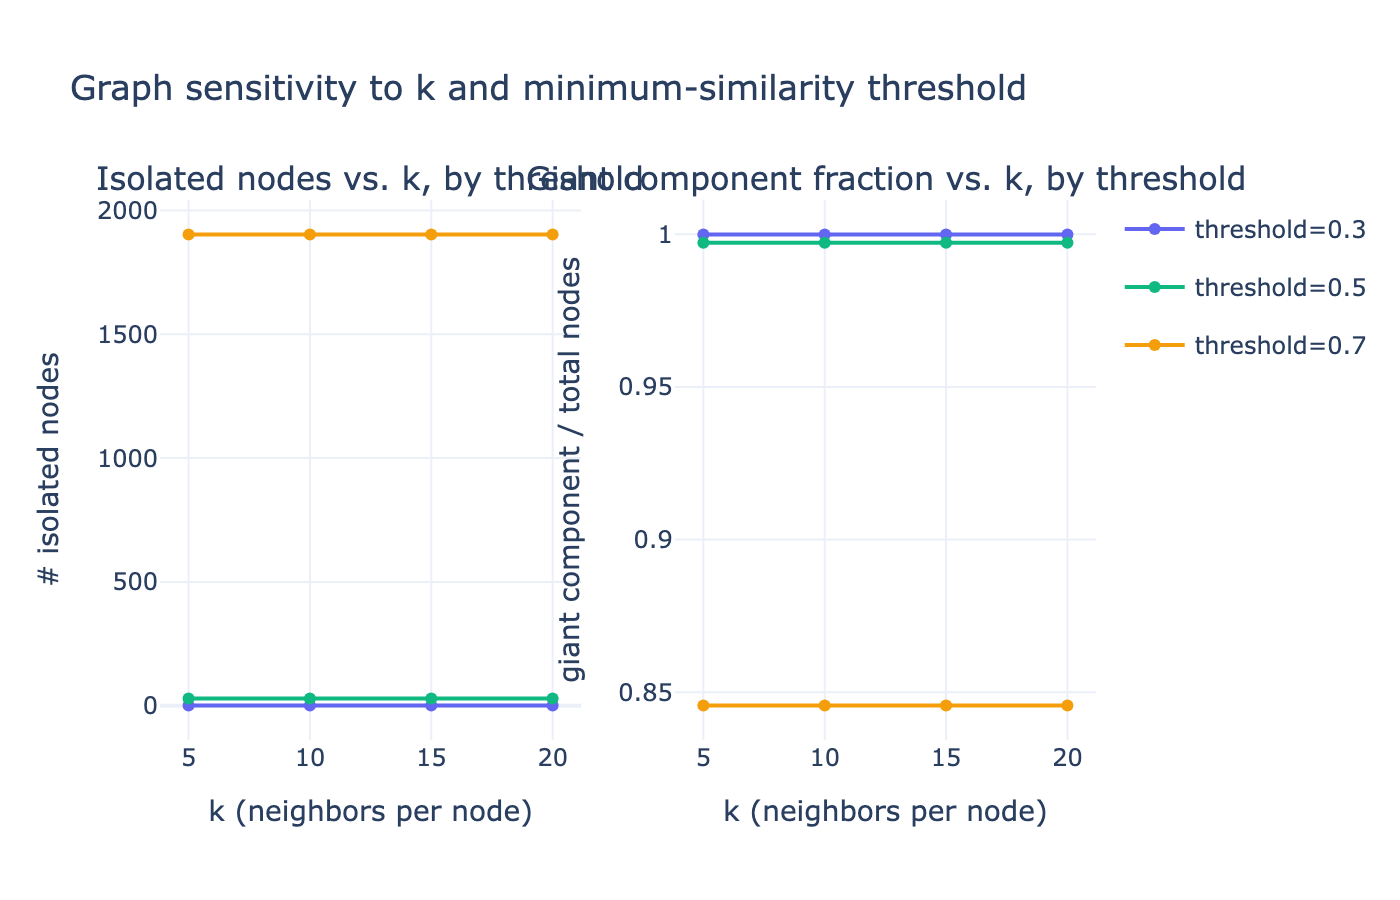
\includegraphics[width=\textwidth]{../../artifacts/week12/week12_sensitivity_sweep.png}
  \caption{Isolated-node count and giant-component fraction as functions of $k$, grouped by
  minimum-similarity threshold.}
  \label{fig:sweep}
\end{figure}

\paragraph{Key observation.} For a fixed threshold, the isolated-node count is \emph{constant}
across all values of $k$ (1 at threshold$=0.3$, 29 at threshold$=0.5$, 1,903 at threshold$=0.7$).
This is because isolation is driven by whether a node's single closest neighbor clears the
threshold at all --- if the top-1 neighbor's similarity already falls below the threshold, looking
at more neighbors ($k$) cannot produce a qualifying edge. The threshold, not $k$, controls
connectivity; $k$ mainly controls how many \emph{additional} edges accumulate once a node is
already connected.

%% ------------------------------------------------------------------
\section{Chosen Configuration and Validity Checks}
%% ------------------------------------------------------------------

Threshold$=0.7$ strands 1,903 nodes (14.4\%) even at $k=20$ --- too strict, since most real
co-rating similarity signal in this 50-dimensional space falls below 0.7. Threshold$=0.3$ is
already near-fully-connected at $k=10$ (99.99\% giant component, only 1 isolated node) --- too
permissive, approaching a near-complete graph and defeating the purpose of a sparse structural
graph.

\textbf{Chosen configuration: $k=15$, min\_similarity$=0.5$.} This keeps the giant component
covering the large majority of nodes (99.72\%) while still discarding most low-similarity pairs
(sparsity 0.179\%), and matches how the Week~10 \texttt{content\_cosine} /
\texttt{svd\_collaborative} recommenders already treat similarity --- same latent space, same
metric.

\begin{table}[H]
\centering
\caption{Validity checks at the chosen configuration}
\begin{tabular}{ll}
\toprule
\textbf{Check} & \textbf{Result} \\
\midrule
Edge sparsity & 0.179\% of all possible undirected pairs --- sparse by design \\
Isolated nodes & 29 / 13,176 (0.22\%) \\
Connected components & 33 (one giant component + 32 small fragments) \\
Giant component coverage & 13,139 / 13,176 nodes (99.72\%) \\
Sensitivity & Section~\ref{sec:sweep} --- connectivity is threshold-driven, not one lucky $k$ \\
\bottomrule
\end{tabular}
\end{table}

%% ------------------------------------------------------------------
\section{Centrality Measures}
%% ------------------------------------------------------------------

Degree, weighted degree, and PageRank are computed on the full graph. Eigenvector centrality is
undefined on disconnected graphs (\texttt{networkx} raises \texttt{AmbiguousSolution}), so it is
computed on the giant connected component only, with 0 assigned to the 37 nodes outside it --- those
nodes have no path into the component's dominant eigenvector by construction, so 0 is the correct
value, not a missing one. Exact betweenness centrality is $O(V\cdot E)$ and infeasible at this scale
(13,176 nodes, 155,331 edges); an approximate betweenness is computed instead using a random sample
of 500 source nodes (\texttt{networkx}'s native \texttt{k} parameter), with edge distance defined as
$1 - \text{similarity}$.

\begin{table}[H]
\centering
\caption{Top 10 movies by PageRank, with degree, weighted degree, and popularity/model rank (out of 13,176)}
\label{tab:top_pagerank}
\begin{tabular}{lrrrrr}
\toprule
\textbf{Movie} & \textbf{PageRank} & \textbf{Degree} & \textbf{Wtd.\ degree} & \textbf{Pop.\ rank} & \textbf{Model-rec.\ rank} \\
\midrule
L'Atalante (1934)            & 0.000265 & 107 & 100.32 & 6,351  & 3,855 \\
The Lazarus Effect (2015)    & 0.000261 &  96 &  85.01 & 7,985  & 5,182 \\
Viridiana (1961)             & 0.000247 & 101 &  95.56 & 5,592  &   916 \\
Day of Wrath (1943)          & 0.000237 &  94 &  88.33 & 8,052  & 3,535 \\
Perfect Stranger (2007)      & 0.000230 &  82 &  68.94 & 6,044  & 1,160 \\
Untraceable (2008)           & 0.000228 &  81 &  66.64 & 5,594  & 2,035 \\
The Reaping (2007)           & 0.000226 &  82 &  70.13 & 5,950  & 2,693 \\
Pickpocket (1959)            & 0.000223 &  90 &  84.13 & 6,120  & 1,033 \\
I Know Who Killed Me (2007)  & 0.000223 &  79 &  70.20 & 7,632  & 5,576 \\
Devil's Knot (2013)          & 0.000217 &  77 &  61.85 & 10,766 & 6,029 \\
\bottomrule
\end{tabular}
\end{table}

\paragraph{Key finding.} None of the top-10 PageRank movies rank in the popularity top-1,000 ---
the highest is L'Atalante at popularity rank 6,351 out of 13,176 (bottom half of the catalog). High
PageRank here means a movie sits in a densely-interconnected neighborhood of the similarity
structure (reachable through many strong-similarity chains), which is a structurally different
property from being widely rated.

%% ------------------------------------------------------------------
\section{Comparison: Graph Ranking vs.\ Popularity vs.\ Model-Based Ranking}
\label{sec:comparison}
%% ------------------------------------------------------------------

Three independent rankings over the same 13,176-node set:

\begin{itemize}[nosep]
  \item \textbf{Popularity ranking}: rank by \texttt{rating\_count} (Week~10
    \texttt{week10\_popularity\_global.csv}) --- ``how many people rated this.''
  \item \textbf{Model-based ranking}: rank by \emph{recommendation in-degree} --- how many times a
    movie appears inside another movie's Week~10 SVD top-20 recommendation list. This is a
    directed, model-derived signal distinct from the graph's undirected similarity edges.
  \item \textbf{Graph ranking}: rank by PageRank on the Week~12 similarity graph.
\end{itemize}

\begin{table}[H]
\centering
\caption{Spearman rank correlations between the three ranking signals}
\begin{tabular}{lr}
\toprule
\textbf{Comparison} & \textbf{Spearman $\rho$} \\
\midrule
Popularity vs.\ graph PageRank & \textbf{0.313} \\
Model rec.\ in-degree vs.\ graph PageRank & \textbf{0.578} \\
Popularity vs.\ model rec.\ in-degree & 0.785 \\
\bottomrule
\end{tabular}
\end{table}

\begin{figure}[H]
  \centering
  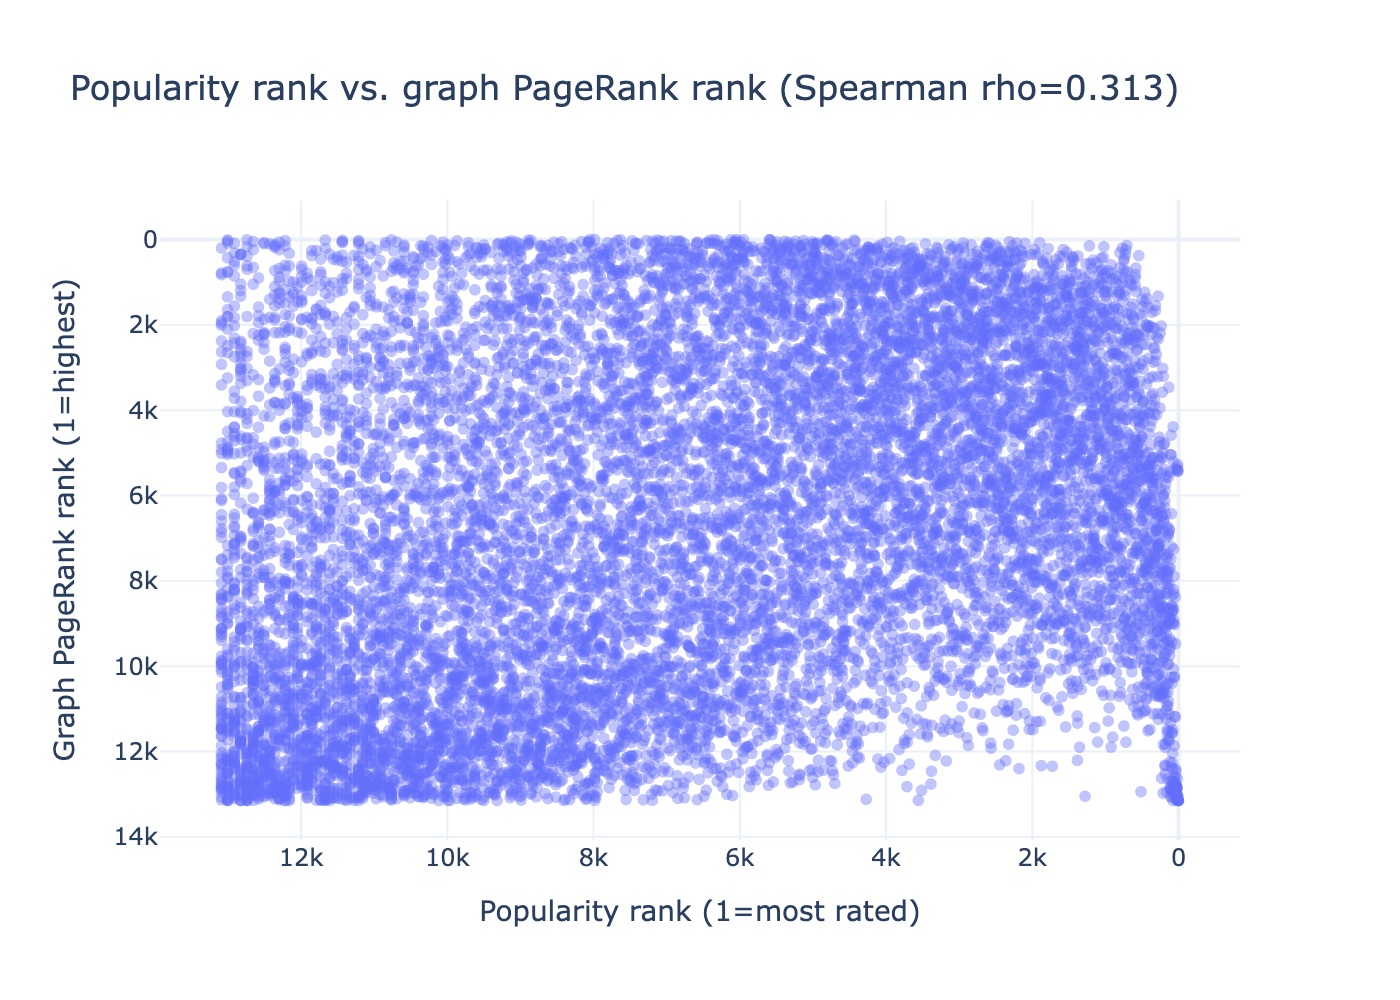
\includegraphics[width=0.85\textwidth]{../../artifacts/week12/week12_popularity_vs_pagerank.png}
  \caption{Popularity rank vs.\ graph PageRank rank (Spearman $\rho=0.313$). Points scatter widely
  around the diagonal, showing the two rankings diverge substantially.}
  \label{fig:pop_vs_pagerank}
\end{figure}

Popularity and the model's recommendation in-degree are strongly correlated ($\rho=0.785$) ---
both are, in different ways, proxies for how mainstream a movie is. Graph PageRank correlates much
more weakly with popularity ($\rho=0.313$) and moderately with model in-degree ($\rho=0.578$): the
similarity graph surfaces a partially different signal --- structural embeddedness in the SVD
similarity space --- that is only loosely tied to how many people rated a movie.

%% ------------------------------------------------------------------
\section{Interpretation Note: What Graph Structure Means, and Does Not Mean}
%% ------------------------------------------------------------------

\textbf{What it means}: an edge between two movies indicates that, in the space learned by the
Week~10 SVD factorization of the user-rating matrix, the two movies have highly correlated rating
patterns across the user base --- people who rate one in a particular direction tend to rate the
other similarly. High PageRank means a movie sits in a densely-interconnected neighborhood of this
similarity structure: not just similar to a few movies, but reachable through many short chains of
strong similarity.

\textbf{What it does not mean}:
\begin{itemize}[nosep]
  \item It is \textbf{not} a claim about shared plot, cast, or genre --- the graph is built purely
    from rating co-occurrence, not content features. Two movies can be structurally central
    neighbors while sharing no genre tag.
  \item High PageRank is \textbf{not} the same as ``popular'' --- $\rho=0.313$ is positive but far
    from 1: the graph surfaces movies that are structurally embedded in the similarity space
    without necessarily being the most-rated movies overall, and vice versa.
  \item The graph is \textbf{not directed} and does not encode ``recommend $A$ because of $B$'' ---
    that asymmetric signal is captured separately by the Week~10 recommendation lists
    (\texttt{model\_rec\_indegree}) used for comparison above.
  \item The similarity signal inherits whatever rating biases exist in MovieLens (predominantly
    English-language, enthusiast-skewed userbase); it should not be read as a universal notion of
    movie similarity.
  \item Isolated nodes and small disconnected components are not ``unrelated'' movies in general
    --- they are movies whose rating pattern did not clear the chosen similarity threshold against
    any node's top-15 neighbors, which can also reflect a small or unusual rater population for
    that title.
\end{itemize}

%% ------------------------------------------------------------------
\section{Subgraph Sampling for the 3D Web Visualization}
%% ------------------------------------------------------------------

Drawing all 13,176 nodes in a browser-based 3D scene is neither readable nor performant, so a
\textbf{connected} subgraph of 400 nodes was sampled for the interactive viewer (\texttt{web/})
using hub-expansion sampling: start from the 40 highest-PageRank nodes in the giant component
(structural hubs), then greedily grow the sample by always adding the unselected node with the
strongest edge weight to an already-selected node. Because every added node is attached by
construction, the sampled subgraph has \textbf{no isolated nodes}, unlike a uniform-random node
sample with an induced-edge cut, which typically strands many isolated points.

\begin{table}[H]
\centering
\caption{Full graph vs.\ sampled subgraph used by the web viewer}
\begin{tabular}{lrr}
\toprule
 & \textbf{Full graph} & \textbf{Sampled subgraph} \\
\midrule
Nodes & 13,176 & 400 \\
Edges & 155,331 & 3,334 \\
Isolated nodes & 29 & 0 (by construction) \\
\bottomrule
\end{tabular}
\end{table}

The sampled subgraph is exported to \texttt{artifacts/week12/movie\_graph\_viz.json} and copied to
\texttt{web/public/movie\_graph.json}, where node metadata (title, genres, IMDb/TMDb links,
PageRank, degree, cluster ID) drives the interactive viewer. Poster URLs are filled in separately
by \texttt{scripts/fetch\_posters.py} via the TMDb API, for exactly this sampled set of movies.

%% ------------------------------------------------------------------
\section{What Worked and What Did Not}
%% ------------------------------------------------------------------

\paragraph{What worked.}
\begin{itemize}[nosep]
  \item Reusing the Week~10 SVD item-factor space as the graph's edge weight keeps the graph
    analysis connected to an existing, already-validated signal instead of introducing an
    unrelated ad hoc similarity metric.
  \item The sensitivity sweep cleanly separates the role of $k$ (marginal edge accumulation) from
    the role of the similarity threshold (connectivity), which made the configuration choice
    defensible rather than arbitrary.
  \item Hub-expansion sampling produced a fully connected, hub-anchored 400-node subgraph suitable
    for a real-time 3D viewer, with zero isolated nodes.
\end{itemize}

\paragraph{What did not work.}
\begin{itemize}[nosep]
  \item \textbf{Eigenvector centrality} is undefined outside the giant component; 37 nodes
    necessarily receive a 0 that reflects ``no path into the dominant eigenvector,'' not ``zero
    centrality'' in an absolute sense --- this distinction has to be stated explicitly or it reads
    as a missing value.
  \item \textbf{Betweenness centrality} could not be computed exactly at this scale (13,176 nodes,
    155,331 edges); the 500-source approximation trades precision for tractability and should not
    be read as an exact ranking.
  \item \textbf{Weak correlation with popularity} ($\rho=0.313$) means graph PageRank alone is a
    poor stand-in for ``movies most people already know'' --- it answers a different question
    (structural embeddedness), not ``what should the homepage show a new user.''
\end{itemize}

%% ------------------------------------------------------------------
\section{Ethics and Access Note}
%% ------------------------------------------------------------------

\begin{itemize}[nosep]
  \item \textbf{Data source}: GroupLens MovieLens~25M public release (research license).
  \item \textbf{Access}: Educational and research use; raw data not redistributed.
  \item \textbf{Personal data risk}: all user identifiers are anonymized integer IDs.
  \item \textbf{Mitigation}: the graph is built entirely at the movie level from aggregate SVD item
    factors; no individual user rating history or user identifier is exposed by any node, edge, or
    centrality score in this analysis.
\end{itemize}

%% ------------------------------------------------------------------
\section{Reproducibility}
%% ------------------------------------------------------------------

Run the notebook after the Week~10 artifacts exist:
\begin{enumerate}[nosep]
  \item \texttt{notebooks/week12/week12\_graph\_analytics.ipynb}
\end{enumerate}

Then, to refresh the web viewer's data:
\begin{enumerate}[nosep]
  \setcounter{enumi}{1}
  \item \texttt{python scripts/fetch\_posters.py} --- populates \texttt{posterUrl} for the
    $\approx$400 sampled movies via the TMDb API.
  \item Copy \texttt{artifacts/week12/movie\_graph\_viz.json} to
    \texttt{web/public/movie\_graph.json}.
\end{enumerate}

\begin{table}[H]
\centering
\caption{Key parameters for reproducibility}
\begin{tabular}{ll}
\toprule
\textbf{Parameter} & \textbf{Value} \\
\midrule
Node definition & Movie with $\geq50$ ratings (has a Week~10 SVD item factor) \\
Candidate nodes & 13,176 \\
Similarity metric & Cosine, on 50-dim Week~10 SVD item factors \\
Chosen $k$ (neighbors per node) & 15 \\
Chosen minimum similarity & 0.5 \\
Betweenness sample size & 500 \\
Subgraph sample size (web viewer) & 400 nodes / 3,334 edges \\
Hub seeds for sampling & 40 (highest PageRank in giant component) \\
Random state & 42 \\
\bottomrule
\end{tabular}
\end{table}

%% ------------------------------------------------------------------
\section{Conclusion}
%% ------------------------------------------------------------------

Week~12 is complete. A 13,176-node, 155,331-edge item-item similarity graph was built directly from
the Week~10 SVD item-factor space, validated with a joint sensitivity sweep over $k$ and similarity
threshold, and analyzed with degree, weighted degree, PageRank, eigenvector, and approximate
betweenness centrality.

\begin{itemize}[nosep]
  \item The chosen configuration ($k=15$, min\_similarity$=0.5$) yields a giant component covering
    99.72\% of nodes, and the sweep shows this connectivity is driven by the threshold, not a
    lucky choice of $k$.
  \item Graph PageRank correlates only weakly with popularity ($\rho=0.313$) and moderately with
    the Week~10 model's recommendation in-degree ($\rho=0.578$): structural centrality in the
    similarity graph is a genuinely different signal from ``most-rated'' or ``most-recommended,''
    not a relabeling of either.
  \item The interpretation note makes explicit what the graph does and does not license: it
    reflects rating co-occurrence, not content similarity; it is undirected and does not encode
    asymmetric recommendation; and it inherits MovieLens's own rating-population biases.
  \item A connected, hub-anchored 400-node subgraph was sampled and exported to drive the
    interactive 3D MovieLens Discovery viewer (\texttt{web/}), completing the pipeline from raw
    ratings through representation, clustering, recommendation, and now graph structure.
\end{itemize}

\end{document}
